\documentclass[11pt,a4paper,titlepage]{article}
\usepackage[utf8]{inputenc}
\usepackage{amssymb}
\usepackage[english,polish]{babel}
\usepackage[T1]{fontenc}
\usepackage{polski}
%\usepackage[math,light]{anttor}
\usepackage[light]{anttor}
\usepackage{amsmath}
\usepackage{amsfonts}
\usepackage{graphicx}
\usepackage{siunitx}
%\usepackage{subcaption}
\usepackage{sidecap}
%\usepackage{wrapfig}
\usepackage{epstopdf}
\usepackage{booktabs}
\usepackage{forloop}
\usepackage[left=3cm,right=3cm,top=3cm,bottom=3cm]{geometry}
\usepackage[framed,numbered,autolinebreaks]{mcode}
\usepackage[colorlinks=false,urlcolor=blue,citecolor=green]{hyperref}
\usepackage{fancyhdr}
\usepackage{lastpage}
\usepackage{array}
\usepackage{hhline}
\usepackage{svg}
\usepackage{multirow}
\usepackage{enumerate}%[I], numerki, [(a)]
\usepackage{float}
%\usepackage{courier}
%ustawienie poziomów wypunktowania do wyboru: $\bullet$, $\cdot$, $\diamond$, $-$, $\ast$ and $\circ$ 
\renewcommand{\labelitemi}{$\diamond$}
\renewcommand{\labelitemii}{$\bullet$}
\renewcommand{\labelitemiii}{$-$}
\renewcommand{\labelitemiv}{$\ast$}

%Figure numbering
\usepackage{chngcntr}
\counterwithin{figure}{section}
\counterwithin{equation}{section}

\newcommand*{\captionsource}[2]{%
  \caption[{#1}]{%
    #1%
    \\\hspace{\linewidth}%
    \textbf{Źródło:} #2%
  }%
}

\AtBeginDocument{

	\renewcommand{\tablename}{Tabela}

	\renewcommand{\figurename}{Rys.}
}

%tabelki
\usepackage{tabularx}
\newcolumntype{A}{>{\centering\arraybackslash}X}
\newcolumntype{B}{>{\centering\arraybackslash} m{0.4\textwidth} }

% --- < bibliografia > ---
\usepackage[
style=numeric,
sorting=none,
% Zastosuj styl wpisu bibliograficznego właściwy językowi publikacji.
language=auto,
autolang=other,
% Zapisuj datę dostępu do strony WWW w formacie RRRR-MM-DD.
urldate=edtf,
seconds=true,
% Nie dodawaj numerów stron, na których występuje cytowanie.
backref=false,
% Podawaj ISBN.
isbn=true,
% Nie podawaj URL-i, o ile nie jest to konieczne.
url=false,
% Ustawienia związane z polskimi normami dla bibliografii.
maxbibnames=3,
% Jeżeli używamy BibTeXa:
backend=biber
]{biblatex}
% --- < bibliografia > --- Koniec

\usepackage{csquotes}
\DeclareQuoteAlias{croatian}{polish} % Ponieważ `csquotes` nie posiada polskiego stylu, można skorzystać z mocno zbliżonego stylu chorwackiego.

\addbibresource{bibliografia.bib}

\pagestyle{fancy}
\fancyhf{}
\fancyhead[R]{Rozpoznawanie obiektów na obrazach zdarzeniowych}
\fancyfoot[R]{Wieloprocesorowe Systemy Wizyjne}
\fancyhead[L]{M. Kowalczyk i J. Piechota}     
\fancyfoot[L]{Strona \thepage \hspace{1pt} z\hspace{1pt} \pageref*{LastPage}}    
\renewcommand{\headrulewidth}{1pt}
\renewcommand{\footrulewidth}{1pt}

\begin{document}
\begin{titlepage}

\newcommand{\HRule}{\rule{\linewidth}{0.5mm}} % Defines a new command for the horizontal lines, change thickness here

\center % Center everything on the page
 
%----------------------------------------------------------------------------------------
%	HEADING SECTIONS
%----------------------------------------------------------------------------------------

\textsc{\LARGE Akademia Górniczo - Hutnicza im. Stanisława Staszica w Krakowie}\\[0.5cm]

\includegraphics[scale=0.6]{agh}\\[1cm] % Name of your university/college
\textsc{\Large Wydział Elektrotechniki, Automatyki, Informatyki i Inżynierii Biomedycznej}\\[0.5cm] % Major heading such as course name
\textsc{\large Kierunek: Automatyka i robotyka}\\[0.5cm] % Minor heading such as course title

%----------------------------------------------------------------------------------------
%	TITLE SECTION
%----------------------------------------------------------------------------------------

\HRule \\[0.4cm]
{ \huge \bfseries Wieloprocesorowe Systemy Wizyjne\\[1cm]Rozpoznawanie obiektów na obrazach w reprezentacji zdarzeniowej}\\[0.4cm] % Title of your document
\HRule \\[1cm]%[3.5cm]
 


%----------------------------------------------------------------------------------------
%	DATE SECTION
%----------------------------------------------------------------------------------------

{\large grudzień 2017}\\[1.5cm] % Date, change the \today to a set date if you want to be precise

%----------------------------------------------------------------------------------------
%	LOGO SECTION
%----------------------------------------------------------------------------------------

%
\includegraphics[height=70mm]{agh.jpg}%\\[1cm] % Include a department/university logo - this will require the graphicx package
%----------------------------------------------------------------------------------------
%	AUTHOR SECTION
%----------------------------------------------------------------------------------------

\begin{flushleft}
\Large
\emph{Wykonali:}\\
Marcin Kowalczyk\\
Jadwiga Piechota\\[1cm]

% If you don't want a supervisor, uncomment the two lines below and remove the section above
 \emph{Prowadzący:}\\
dr inż. Mirosław Jabłoński\\[3cm] % Your name
 
\end{flushleft}
%----------------------------------------------------------------------------------------
\end{titlepage}
\clearpage
\setcounter{page}{2}

\begin{center}
\begin{figure}[H]
	\centering
	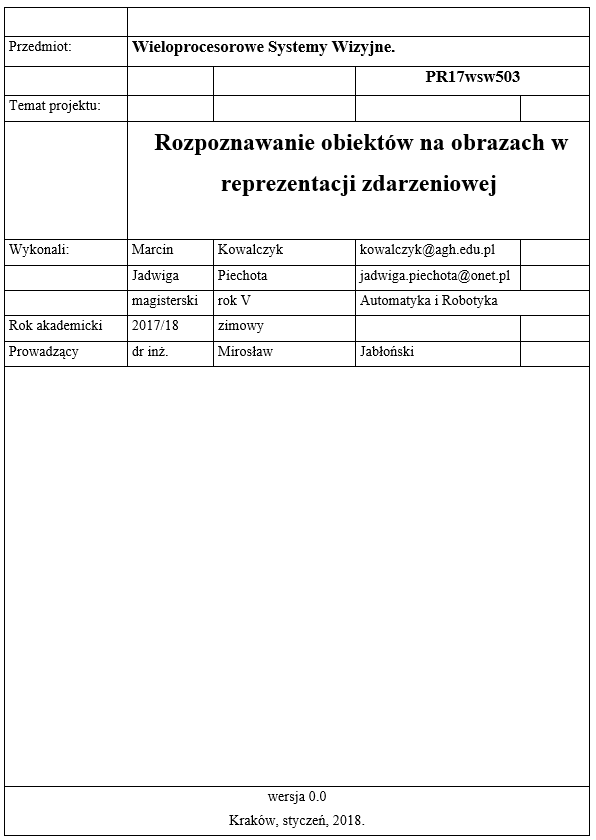
\includegraphics[scale=1]{obrazki/wstep}
\end{figure}
\end{center}

\section*{Streszczenie}
Celem projektu było zaprojektowanie i implementacja sieci neuronowej do rozpoznawania obiektów na obrazach w reprezentacji zdarzeniowej. Skorzystano z bazy danych \textit{MNIST-DVS}, która zawiera obrazy cyfr zapisane w tej reprezentacji. W celu zmniejszenia ilości danych potrzebnych do przetworzenia oraz poprawy jakości obrazów wykonano proste przetwarzanie wstępne. Dane zostały następnie przekonwertowane do postaci, która może posłużyć do uczenia sieci neuronowej. Na koniec sprawdzono skuteczność w zależności od wielkości sieci.
 
\clearpage
\tableofcontents
\clearpage

\section{Wstęp}
\label{sec:wstep}

\subsection{Cel projektu}
\label{sub:celprojektu}

Celem projektu jest implementacja rozwiązania pozwalającego na rozpoznawanie obiektów na obrazach w reprezentacji zdarzeniowej. Idea reprezentacji zdarzeniowej polega na zaznaczaniu pikseli, dla których nastąpiła pewna zmiana w obrazie wejściowym kamery. Współrzędne wraz z typem zmiany (wzrost lub spadek wartości piksela) tego piksela następnie są wysyłane do zewnętrznego urządzenia, które przetwarza te dane. Metoda ta pozwala na zmniejszenie ilości danych, które potrzebne są do przesłanie z kamery i przetworzenia w innym urządzeniu. Projekt zakłada, że zapisane dane z reprezentacji zdarzeniowej są następnie przetworzone przez sieć neuronową zaimplementowaną w~programie \textit{MATLAB}.


\subsection{Proponowane rozwiązanie}
\label{sub:proponowanerozwiazanie}

Zaproponowane i sprawdzone rozwiązanie wymaga wstępnego przetworzenia zarejestrowanych danych. Polega ono na agregowaniu współrzędnych pikseli z \(10 \si{us}\). Dane te następnie formatowane jako obraz o rozmiarze \(40\times40\si{px}\) oraz jako wektor, którego kolejne elementy są kolejnymi elementami stworzonego obrazu. Stworzone w ten sposób wektory są danymi wejściowymi sieci neuronowej. Dane wyjściowe są zapisywane w~postaci wektora one-hot. Jest to wektor, który ma na jednym miejscu jedynkę, a na pozostałych zera. Tak przygotowane dane poddane są uczeniu z nauczycielem przez głęboką sieć neuronową, ponieważ rozważany problem jest problemem klasyfikacji. Wykorzystane narzędzia to funkcje do uczenia sieci neuronowej z wykorzystaniem autoenkodera zawarte w narzędziu programu \textit{MATLAB - Neural Network Toolbox}. Użyte zostały dwa autoenkodery, które następnie wspólnie z warstwą wyjściową typu \textit{softmax} tworzą całą głęboką sieć neuronową. Zbiór wejściowy podzielono na trzy części: dane do uczenia, walidacji i testowania. W kontekście alternatywnego rozwiązania okazało się prostsze w implementacji. Uzyskano zadowalające efekty, zatem zaproponowane rozwiązanie jest skuteczne i może być z powodzeniem wykorzystywane w procesie rozpoznawania cyfr.


\subsection{Alternatywne rozwiązania}
\label{sub:alternatywnerozwiazania}

Alternatywne rozwiązanie zakładało implementację z użyciem impulsowych sieci neuronowych. Sieci te stanowią stosunkowo nowe podejście, a sposób działania bardziej zbliżony do rzeczywistych procesów zachodzących w mózgu. Lepiej też naśladują naturalne neurony. Bazują na sposobie przekazywania przez nie informacji, jaką jest impuls elektryczny. Jak zostało napisane w \cite{impuls2}, sieci te lepiej nadają się do zadań dynamicznych.
Podejście to wydaje się być idealnym rozwiązaniem do postawionego tu problemu. Naturalne neurony generują impulsy, które są przekazywane dalej \cite{impuls}. Tutaj sieć reagowałaby na impulsy, czyli zmiany położenia obrazu wejściowego, tzw. zdarzenia. W~dostępnej bazie każda kolejna dana generuje nowe zdarzenia, a więc impulsy, wynikające ze zmiany położenia badanego obiektu. 
Pomimo faktu, iż sieć ta idealnie nadałaby się do postawionego problemu, nie zdecydowano się na jej implementację. To stosunkowo nowe podejście, dlatego nie znaleziono gotowych bibliotek, które mogłyby ułatwić proces uczenia, ponieważ napisanie funkcji do uczenia tej sieci to temat obszerny i wykraczający poza możliwości zadania projektowego. Dodatkowo do symulacji tego typu sieci potrzebna jest duża moc obliczeniowa \cite{impuls2}, co wiąże się z koniecznością dostępu do komputera spełniającego pewne wymagania sprzętowe.
\section{Analiza złożoności i estymacja zapotrzebowania na zasoby}
\label{sub:analiza}

Zadanie projektowe zostało podzielone na dwie części. Pierwsza z nich dotyczyła odpowiedniego przygotowania danych, czyli wybrania odpowiednich zdarzeń z bazy \textit{MNIST-DVS} i dostosowania ich do aktualnych potrzeb. Dane te zostały następnie użyte podczas właściwego działania algorytmu, czyli uczenia i testowania sieci neuronowej.

\subsection{Przygotowanie danych}
\label{sub:przygotowanie}

Cała baza \cite{baza} zawierała bardzo dużo informacji. Nie było konieczności użycia tak dużej liczby wartości, dlatego zdecydowano się na wybranie około 10\%. Liczba ta okazała się wystarczająca do zobrazowania wyników istotnych z punktu widzenia założonych celów.
W celu znalezienia zbioru uczącego, napisano skrypt w programie \textit{MATLAB 2017b}. Ta część zadania nie wymagała specjalnych zasobów obliczeniowych. Podstawowe wymagania systemowo - sprzętowe, potrzebne do poprawnego działania programu \textit{MATLAB 2017b}, znalezione w \cite{wymagania_Matlab}, są następujące:

\begin{itemize}
\item system operacyjny: Windows 7 SP1 / Windows 8.1 / Windows 10
\item procesor: Intel lub AMD x86-64 (rekomendowane wsparcie dla instrukcji AVX2)
\item dysk: 4 - 6 Gb dla instalacji, 2 Gb wolnego miejsca dla prawidłowego działania programu
\item RAM: co najmniej 2 Gb
\item grafika: nie jest wymagana żadna konkretna karta graficzna, jednak polecana to taka, która ma wsparcie dla OpenGL 3.3 z 1 Gb pamięci GPU.
\end{itemize}

Zasoby pamięciowe, jakie dodatkowo musi posiadać komputer PC, na którym działa program, muszą pomieścić oryginalną bazę, która zajmuje około 9 Gb miejsca. Jednak już po przetworzeniu jej przez \textit{MATLAB} zajmuje dużo mniej miejsca - to około 200 Mb.
Aplikacja musi poradzić sobie z dużą ilością danych - na bazę składa się około 100 000 plików,  przedstawiających zdarzenia przypadające na pewne przesunięcie danej liczby. Pliki te są zapisane w formacie .aedat, stworzonym przez twórców \cite{MNIST_DVS}. Autorzy stworzyli specjalny skrypt, który pozwala na zamianę formatu .aedat na format, który może być odczytany i dalej przetwarzany przez \textit{MATLAB} (format .mat). Wymaga to wykonaniu dodatkowego szeregu instrukcji przy każdorazowym przetwarzaniu pliku z bazy, a wyniki tu generowane są przedstawione w formacie double. To wszystko powoduje dość długi czas trwania obliczeń, dlatego im lepsze parametry ma komputer PC, na którym wykonywane są obliczenia, tym wyniki uzyskiwane są sprawniej. Po wykonaniu obliczeń, uzyskuje się dwie macierze, wykorzystywane później do uczenia sieci. W obu wartościami są liczby boolean. Ponieważ nie ma tutaj żadnych zależności z pozostałymi modułami (baza została przygotowana wcześniej i nie koliduje z procesem uczącym), nie ma znaczenia na jakim komputerze będą wykonywane obliczenia. Możliwości sprzętowe powodują jednak, że efektywność pracy rośnie.

\subsection{Uczenie sieci neuronowej}
\label{sub:uczenie}

Właściwa część algorytmu, czyli uczenie i testowanie sieci neuronowej została również wykonana w programie \textit{MATLAB 2017b}. Wymagania sprzętowo - programowe są tu więc identyczne co te, wymienione w sekcji \ref{sub:przygotowanie}. Jednak tutaj zastosowano dwa różne podejścia do tematu.

Pierwsze podejście zakładało użycie gotowego GUI programu \textit{MATLAB - Neural Network Toolbox}, stworzonego do uczenia i testowania sieci neuronowej. Jedynym wymaganiem był tu dostęp do tego narzędzia z poziomu programu \textit{MATLAB}. 

Drugie podejście polegało na stworzeniu sieci neuronowej za pomocą funkcji programu \textit{MATLAB}. Dodatkowo, w celu przyspieszenia obliczeń, wykorzystano tutaj GPU (z ang. \textit{ graphics processing unit}). Aby taki algorytm mógł działać, niezbędna jest tutaj karta graficzna NVIDIA wyposażona w jednostkę obliczeniową, obsługująca architekturę obliczeniową CUDA (z ang. \textit{Compute Unified Device Architecture}). Takie podejście jest uzasadnione, ponieważ uczenie sieci neuronowych to proces równoległy. Zatem zwiększenie zrównoleglenia obliczeń poprzez użycie dodatkowego procesora znacznie usprawni przebieg działania i spowoduje, że testowanie, polegające na wielokrotnym uczeniu sieci z różnymi parametrami będzie szybsze, a cały proces bardziej efektywny. Wydajność w tym przypadku wzrasta w znacznym stopniu.

W obu podejściach jako wektory wejściowe podane są macierze:

\begin{itemize}
\item danych -  94 490 $\times$ 1600
\item wyjść -  94 490 $\times$ 10 
\end{itemize}
W obu przypadkach w pierwszym podejściu były to wartości logiczne, w drugim zostały zapisane jako typ \textit{double}.
\section{Koncepcja proponowanego rozwiązania}
\label{sub:koncepcja}

Pierwsza część pracy polegała na stworzeniu bazy danych, na których następnie można było uczyć sieć neuronową. Jak zostało wspomniane w sekcji \ref{sub:analiza}, około 10\% danych dostarczonych przez autorów bazy \textit{MNIST-DVS} w źródle \cite{MNIST_DVS} zostało wykorzystanych w niniejszej pracy. Ponieważ rozważano dwie koncepcje, dane zostały przygotowane do realizacji obu w podobny sposób, jednak na końcu zostały zapisane w innej formie, co zostanie omówione w późniejszej części rozdziału.

Dane zostały wybrane w sposób losowy, odrzucono tylko początkowe wartości, które mogłyby być nieco zaszumione i wprowadzać niepotrzebne rozbieżności. Mając już tak przygotowany zestaw danych, zauważono pewną powtarzalność w przedstawianiu zdarzeń. Otóż zdarzenia przedstawiające zmianę położenia liczby znajdują się w podobnym miejscu (jak już zostało wspomniane, nie cały zestaw danych, czyli zbiór zdarzeń został wzięty pod uwagę). Dzięki temu można było znacząco zmniejszyć wymiary danych wejściowych do rozmiaru 40 $\times$ 40. Taki zabieg przyspieszył i tak już zaawansowane obliczenia.
W dalszej kolejności stworzono tablicę wartości boolean o rozmiarze 40 $\times$ 40 i przepisano tam wartość 1 w miejscach, gdzie wystąpiły zdarzenia. W ten sposób powstało 94 490 takich tablic (po około 10 000 na jedną cyfrę). Braki wynikają z błędów twórców bazy \textit{MNIST-DVS}, ale zostały wyeliminowane w procesie działania zaprezentowanego algorytmu. Ponieważ uczenie sieci neuronowej zastosowanej w omawianej metodzie następowało z nauczycielem, potrzebne było stworzenie macierzy wyjść. Macierz do tego utworzona miała tyle wierszy, ile tablic wejściowych, zaś kolumn tyle co cyfr, czyli 10. Wartość 1 w danej kolumnie informowała tu z jaką cyfrą mamy w tym przypadku do czynienia - numer kolumny wskazywał cyfrę pomniejszoną o jeden (pierwsza kolumna dla 0).  

Uczenie sieci odbyło się równolegle na dwa sposoby. Pierwszy wymagał przedstawienia danych w postaci wierszowej. Stworzono więc macierz mającą tyle wierszy, ile danych wejściowych i tyle kolumn, ile wartości przypadało na każdą daną, czyli 1600. Drugi sposób pozwalał na stworzenie tablicy celek. Dane wejściowe były przedstawione w taki sposób, że każda celka była tablicą 40 $\times$ 40, czyli jedną daną. Etykiety stworzono bazując na macierzy wyjść. Każda celka przestawiała tu wektor o rozmiarze 10, w którym na odpowiednim miejscu, oznaczającym daną cyfrę, znajdowała się wartość 1. Synchronizację otrzymano poprzez numer celki w danych wejściowych odpowiadał numerowi celki w tablicy wyjściowej zawierającej etykiety.

Pierwsze podejście uczenia sieci zakładało użycie GUI programu \textit{MATLAB - Neural Network Toolbox}, a dokładnie jego części odpowiedzialnej za rozpoznawanie wzorców i klasyfikację danych - \textit{nprtool}. Po wprowadzeniu tu wartości wejściowych i etykiet, ustala się liczbę neuronów ukrytych i można już przejść do nauki sieci neuronowej. \textit{MATLAB} sam ustala tutaj liczbę danych potrzebnych do uczenia, walidacji i testowania. Program używa tutaj sieci neuronowej z użyciem algorytmu wstecznej propagacji błędów (z ang. \textit{backpropagation}). Algorytm uczenia kończy działanie po udanej sześciokrotnej walidacji. Wyniki testowania można zaobserwować na stworzonych przez GUI statystykach.

Drugie podejście zostało stworzone po to, aby móc zastosować głęboką sieć neuronową. Uczenie tej sieci odbywa się używając macierzy wejściowej i etykiet wyjściowych, czyli jest to uczenie z nauczycielem. Dodatkowo wprowadzone parametry pozwalają na zastosowanie równoległości obliczeń na wielu rdzeniach oraz użycie procesora graficznego GPU. Zastosowanie jest uzasadnione ze względu na dużą liczbę danych wejściowych, co zostało omówione w sekcji \ref{sub:analiza}. To wszystko pozwala na przyspieszenie tego etapu uczenia. Uzasadnione jest tu użycie autoenkodera w celu dodania warstw ukrytych. Użyto tutaj GPU dodając odpowiedni parametr w funkcji \textit{trainAutoencoder}, ustalona została też maksymalna liczba epok. W celu stworzenia pełnej sieci, dodano warstwę wyjściową. Uwzględniając fakt, że jest to problem klasyfikacyjny, stworzono funkcję aktywacji typu \textit{softmax}. Tak nauczoną sieć poddano testowaniu. Wyniki uzyskane nieco różnią się od wyników uzyskanych w podejściu wcześniejszym, co zostanie omówione w sekcji \ref{sub:testowanie}.

%\subsection{Przygotowanie danych}
%\label{sub:przygotowanie}

% schemat blokowy ?
\section{Symulacja i testowanie}
\label{sub:testowanie}



\subsection{Modelowanie i symulacja}
\label{sub:modelowanie}


\subsection{Testowanie a weryfikacja}
\label{sub:weryfikacja}


\section{Rezultaty i wnioski}
\label{sub:rezultaty}



%\subsection{Modelowanie i symulacja}
%\label{sub:modelowanie}



\section{Podsumowanie}
\label{sub:podsumowanie}



\section{DODATEK A: Szczegółowy opis zadania}
\label{sub:dodatekA}

\subsection{Specyfikacja projektu}
\label{sub:specyfikacja}

Tematem projektu było rozpoznawanie obiektów na obrazach w reprezentacji zdarzeniowej. Postawione zadanie wymagało znalezienia odpowiednich danych, które zostały przedstawione poprzez następujące po sobie zdarzenia. Podejście to nieco różni się od standardowego, trudno byłby wygenerować zbiór uczący  w ramach realizacji tego zadania, bo to już jest temat na inny projekt. W literaturze poleconej przez prowadzącego znaleziono metodę, której wynikiem była baza \textit{MNIST-DVS}. Baza ta została odnaleziona w \cite{baza} i wykorzystana do uczenia sieci neuronowej. Celem, jaki został postawiony, było nauczenie sieci neuronowej, bazując na zdarzeniowej reprezentacji danych, aby była w~stanie rozpoznać 10 cyfr: 0, 1, 2, 3, 4, 5, 6, 7, 8, 9. Wybór rodzaju sieci oraz platform sprzętowo - programowych prowadzący zostawił autorom projektu. 

\subsection{Szczegółowy opis realizowanych algorytmów przetwarzania danych}
\label{sub:opis}

Sekcja ta będzie rozszerzeniem informacji zawartych już wcześniej w paragrafie \ref{sub:koncepcja}. Zastosowane algorytmy zostaną tu omówione bardziej od strony matematycznej.

\subparagraph{Przygotowanie danych}
\label{sub:przyg}

Przetwarzanie bazy \textit{MNIST-DVS} zostało napisane w programie \textit{MATLAB}. Było to konieczne, ponieważ autorzy artykułu \cite{MNIST_DVS} zastosowali rozszerzenie .aedat. Dostarczyli dodatkowo skrypt \textit{dat2mat}, który pozwalał na zamianę tych danych na pliki z rozszerzeniem .mat, które można już w łatwy sposób podglądnąć i~przetworzyć. W tym przypadku zastosowano przetwarzanie sekwencyjne, tworząc skrypt, który zamieniał rozszerzenie i dostosowywał bazę do realizacji postawionych w projekcie celów.

\subparagraph{Uczenie sieci}
\label{sub:ucz}

Uczenie sieci przebiegało z użyciem wbudowanych funkcji programu \textit{MATLAB}, co znacznie ułatwiło pracę. Dane były przetwarzanie współbieżnie, wykorzystując rdzenie procesora CPU oraz procesor graficzny GPU. Pierwszy sposób, uwzględniający GUI do uczenia sieci neuronowych, używał algorytmu wstecznej propagacji błędów i będzie omówiony w sekcji \ref{sub:wstecz}. Drugi sposób polegał na wykorzystaniu wbudowanych funkcji do uczenia maszynowego i używał głębokich sieci neuronowych do klasyfikacji danych. 

\subparagraph{Algorytm wstecznej propagacji błędów}
\label{sub:wstecz}

To podstawowy algorytm uczenia nienadzorowanego wielowarstwowych sieci neuronowych. Zaletą tej sieci jest to, że wagi można tu wytrenować, znajdując ich optymalny zestaw \cite{back}. Metoda umożliwia modyfikację wag w sieci o architekturze warstwowej, we wszystkich jej warstwach. Po ustaleniu topologii, początkowe wagi są inicjowane tu losowo. Przyjmują bardzo małe wartości. Następnie dla danego wektora uczącego oblicza się odpowiedź sieci, warstwa po warstwie, stosując algorytm spadku gradientowego \cite{back2}. Każdy neuron wyjściowy oblicza swój błąd, który następnie jest propagowany do wcześniejszych warstw. Następnie każdy neuron modyfikuje wagi na podstawie wartości błędu. Dodatkowo jest tu wprowadzona powtarzalność, czyli gdy wszystkie dane wejściowe zostaną już użyte, zmieniana jest ich kolejność i ponownie są wprowadzana do sieci. Proces trwa do momentu zatrzymania się średniego błędu kwadratowego. Jest to proces dość kosztowny obliczeniowo, zwłaszcza kiedy sieć jest rozbudowana.

\subparagraph{Głębokie sieci neuronowe}
\label{sub:glebokie}

Uczenie głębokie sieci neuronowej następuje krok po kroku. Pozwala na stopniowe wyznaczenie wag dla poszczególnych warstw sieci w celu innej reprezentacji cech wspólnych. To poszczególne warstwy reprezentują tu cechy wspólne wzorców uczących i na tej podstawie tworzą reprezentacje bardziej skomplikowanych cech w kolejnych warstwach sieci głębokich. Jest to ulepszona metoda niż wielowarstwowe sieci neuronowe uczone algorytmem propagacji wstecznej, w której w~warstwach oddalonych od wyjścia sieci sieć ma tendencję do dokonywania coraz mniejszych zmian \cite{deep}. Tutaj sieć jest rozbudowywana powoli o kolejne warstwy dopiero wtedy, gdy w~poprzednich warstwach pojawiły się takie cechy. Stosuje się tu sieci typu \textit{auto-encoder}, które używając aproksymacji identycznościowej wykorzystują warstwę ukrytą składającą się z mniejszej ilości neuronów niż ilość wejść lub wyjść z sieci. W przypadku głębokich sieci neuronowych trzeba uważać na to, aby sieć nie dopasowała się zbyt mocno do danych uczących, ponieważ na danych testowych może później niepoprawnie działać.

W przypadku realizacji przestawionego projektu wykorzystano głębokie sieci neuronowe do uczenia nadzorowanego, ponieważ rozważano problem klasyfikacji. Do realizacji głębokiego uczenia użyto tutaj auto-enkoderów, jako funkcja aktywacji posłużyła w~warstwie wyjściowej funkcja typu \textit{softmax}. Dokładny opis procedur znajduje się w~sekcji \ref{sub:dodatekB}.

% literatura

\section{DODATEK B: Dokumentacja techniczna}
\label{sub:dodatekB}

Projekt został napisany w programie \textit{MATLAB 2017b}. Korzystano z gotowego GUI programu \textit{MATLAB - Neural Network Toolbox} oraz innych funkcji z tego \textit{toolbox}. Baza danych potrzebna do realizacji postawionego zadania została pobrana z źródła \cite{baza_down}.

\subsection{Dokumentacja oprogramowania}
\label{sub:dokumentacja}

Wszystkie funkcje użyte na potrzeby zaimplementowania algorytmu zostały zaczerpnięte z gotowych rozwiązań. Opis i dokumentacja techniczna GUI \textit{Neural Network Toolbox} znajduje się w źródle \cite{gui}, zaś do funkcji użytych w procesie tworzenia głębokich sieci neuronowych w źródle \cite{funkcje}.

\noindent Kolejność użytych funkcji przedstawiono na schemacie \ref{fig:flow}. Dokładne omówienie kodu znajduje się poniżej.

\vspace{0.6cm}

\begin{figure}[H]
	\centering
	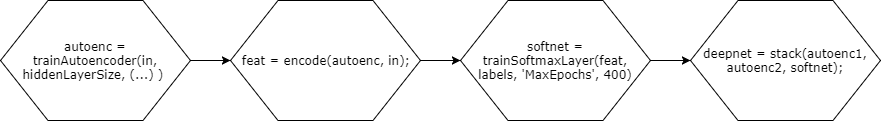
\includegraphics[scale=0.45]{obrazki/flow}
	\caption{\label{fig:subcaption_example}Schemat blokowy użytych funkcji do głębokiego uczenia sieci neuronowej.}{\label{fig:flow}}
\end{figure}

\noindent Funkcja \textit{trainAutoencoder} tworzy ukryte warstwy o zadanej liczbie neuronów. Jako parametry przyjmuje dane wejściowe, ilość ukrytych neuronów oraz parametry określające dynamikę i właściwości wag. Dodatkowo można tu zdecydować, czy obliczenia mają być wykonywane również na procesorze GPU. Funkcja \textit{encode} służy do ekstrakcji cech z~ukrytych warstw, a jako parametry przyjmuje dane wejściowe oraz wynik działania auto-enkodera. Funkcja \textit{trainSoftmaxLayer} tworzy funkcję aktywacji typu softmax, bazując na cechach zwróconych po wywołaniu funkcji \textit{encode} oraz etykietach danych wejściowych. Określa się tutaj także maksymalną liczbę epok. Ostatnia funkcja \textit{stack} układa wszystkie warstwy, łącząc stworzone auto-enkodery oraz warstwę wyjściową. Funkcja ta tworzy głęboką sieć neuronową, która może być już użyta do testowania.


\noindent Dokumentacja techniczna do każdej użytej funkcji znajduje się poniżej.

\vspace{1cm}
\hrule
\vspace{1cm}

\noindent data = dat2mat(['path' '.aedat']);
\vspace{1cm}

\noindent \textit{@file} Skrypt programu \textit{MATLAB} napisany przez twórców\cite{MNIST_DVS} bazy \textit{MNIST-DVS} do zamiany formatu danych .aedat na format .mat akceptowany i widziany przez \textit{MATLAB}.
\\ \textit{@param} ['path' '.aedat'] Ścieżka do danych w formacie .aedat.
\\ \textit{@return} data Wynik działania skryptu. Przedstawienie danych podanych jako parametr w formacie .mat.

\vspace{1cm}
\hrule
\vspace{1cm}

\noindent [trainInd,valInd,testInd] = dividerand(length(images), trainRatio, valRatio, testRatio);
\vspace{1cm}

\noindent \textit{@fn} dividerand Funkcja dzieli określony ciąg liczb na trzy grupy używając losowych indeksów. W przypadku rozważanego algorytmu funkcja umożliwiła losowy podział zbioru wejściowego na zbiór: uczący, walidacyjny i testowy.
\\ \textit{@param} length(images) Liczba określająca wielkość zbioru, który ulega podziałowi. Tu: wielkość bazy danych wejściowych.
\\ \textit{@param} trainRatio Stosunek procentowy udziału danych w zbiorze treningowym. Default = 0.7.
\\ \textit{@param} valRatio Stosunek procentowy udziału danych w zbiorze walidacyjnym. Default = 0.15.
\\ \textit{@param} testRatio Stosunek procentowy udziału danych w zbiorze testowym. Default = 0.15.
\\ \textit{@return} trainInd Wektor indeksów danych treningowych.
\\ \textit{@return} valInd Wektor indeksów danych walidacyjnych.
\\ \textit{@return} testInd Wektor indeksów danych testowych.

\vspace{1cm}
\hrule
\vspace{1cm}

\noindent autoenc1 = trainAutoencoder(images$\_$train,hiddenSize1, ...
\\ \indent   'MaxEpochs',400, ...
\\ \indent   'L2WeightRegularization',0.004, ...
\\ \indent   'SparsityRegularization',4, ...
\\ \indent   'SparsityProportion',0.15, ...
\\ \indent   'ScaleData', false, ...
\\ \indent   'useGPU',true);
\vspace{1cm}

\noindent \textit{@fn} trainAutoencoder Funkcja trenuje auto-enkoder o zadanej liczbie neuronów ukrytych i kluczowych parametrach z punktu widzenia budowy sieci i użycia zasobów sprzętowych.
\\ \textit{@param} images$\_$train Zbiór danych uczących w przypadku pierwszej warstwy ukrytej. W przypadku tworzenia kolejnych warstw (w rozważanym zadaniu użyto dwóch auto-enkoderów) jest to zbiór wyjściowy danych z poprzedniej warstwy ukrytej. Dane powinny być wyrażone w postaci macierzy lub tablicy celek. W każdym z przypadków dane powinny znajdować się w kolumnach bądź poszczególnych celkach o takim samym rozmiarze.
\\ \textit{@param} hiddenSize1 Liczba neuronów w warstwie ukrytej, jest to dodatnia wartość typu integer. Default = 10.
\\ \textit{@param} 'MaxEpochs' Maksymalna liczba epok treningowych, jest to dodatnia wartość typu integer. Default = 1000.
\\ \textit{@param} 'L2WeightRegularization' Współczynnik dla regulacji wag. Regulacja ta pozwala na uniknięcie zbytniego wzrostu wartości wag na rzecz wyjścia. Powoduje wyskalowanie tego parametru w funkcji kosztu. Jest to dodatnia wartość skalarna. Default = 0.001.
\\ \textit{@param} 'SparsityRegularization' Współczynnik kontrolujący wpływ parametru odpowiedzialnego za regulację wartości aktywacji neuronów w funkcji kosztu. Jest to dodatnia wartość skalarna. Default = 1.
\\ \textit{@param} 'SparsityProportion' Wskaźnik określający na ile przykładów danych treningowych ma reagować neuron. Im ta wartość jest mniejsza, tym neuron na mniej danych wejściowych będzie reagował wysokim wyjściem. Jest to dodatnia wartość skalarna z~zakresu 0 - 1. Default = 0.05.
\\ \textit{@param} 'ScaleData' Parametr odpowiedzialny za skalowanie rozmiarem danych w auto-enkoderze automatycznie, co powoduje, że wejścia są replikowane na wyjścia. Przyjmuje wartość true lub false. Default = true.
\\ \textit{@param} 'useGPU' Parametr określający użycie GPU podczas trenowania. Przyjmuje wartość true lub false. Default = false.
\\ \textit{@return} autoenc1 Auto-enkoder stworzony z zadanymi parametrami, wytrenowany za pomocą danych wejściowych images$\_$train.

\vspace{1cm}
\hrule
\vspace{1cm}

\noindent plotWeights(autoenc1);
\vspace{1cm}

\noindent \textit{@fn} plotWeights Funkcja wyświetlająca wagi dla neuronów ukrytych. Funkcja nie zwraca żadnych wartości, ale w wyniku jej działania na ekranie pojawia się wykres.
\\ \textit{@param} autoenc1 Auto-enkoder stworzony i wytrenowany za pomocą funkcji \textit{trainAutoencoder}.

\vspace{1cm}
\hrule
\vspace{1cm}

\noindent feat1 = encode(autoenc1, images$\_$train);
\vspace{1cm}

\noindent \textit{@fn} encode Funkcja tworzy i zwraca zakodowane dane, podane jako parametr, używając wytrenowanego wcześniej auto-enkodera. Dane te mogą być później wykorzystane jako wejście do kolejnych warstw ukrytych lub warstwy wyjściowej.
\\ \textit{@param} autoenc1 Auto-enkoder stworzony i wytrenowany za pomocą funkcji \textit{trainAutoencoder}.
\\ \textit{@param} images$\_$train Zbiór danych uczących w przypadku pierwszej warstwy ukrytej. W przypadku tworzenia kolejnych warstw (w rozważanym zadaniu użyto dwóch auto-enkoderów) jest to zbiór wyjściowy danych z poprzedniej warstwy ukrytej. Dane powinny być wyrażone w postaci macierzy lub tablicy celek. W każdym z przypadków dane powinny znajdować się w kolumnach bądź poszczególnych celkach o takim samym rozmiarze. Format tych danych zależy od tego, na jakim formacie danych trenowany był auto-enkoder.
\\ \textit{@return} feat1 Dane zakodowane za pomocą auto-enkodera i wyrażone w postaci macierzy. To cechy wygenerowane z danych wejściowych. Każda dana reprezentuje osobną kolumnę, ilość wierszy wskazuje na ilość neuronów ukrytych w auto-enkoderze.

\vspace{1cm}
\hrule
\vspace{1cm}

\noindent labels$\_$train$\_$temp{i} = reshape(labels$\_$train{i}, [size$\_$x,size$\_$y]);
\vspace{1cm}

\noindent \textit{@fn} reshape Funkcja powoduje utworzenie nowej tablicy poprzez zmianę wymiarów tablicy już istniejącej.
\\ \textit{@param} labels$\_$train{i} Tablica wzorcowa, która zostaje poddana zmianie rozmiaru.
\\ \textit{@param} [size$\_$x,size$\_$y] Nowy rozmiar tablicy.
\\ \textit{@return} labels$\_$train$\_$temp{i} Miejsce, w którym zostanie zapisana nowa tablica.

\vspace{1cm}
\hrule
\vspace{1cm}

\noindent labels$\_$train3 = cell2mat(labels$\_$train$\_$temp);
\vspace{1cm}

\noindent \textit{@fn} cell2mat Funkcja konwertująca tablicę celek na standardową tablicę podstawowych typów.
\\ \textit{@param} labels$\_$train$\_$temp Tablica celek.
\\ \textit{@return} labels$\_$train3 Tablica standardowa, utworzona z elementów znajdujących się poprzednio w celkach.

\vspace{1cm}
\hrule
\vspace{1cm}

\noindent softnet = trainSoftmaxLayer(feat2, labels$\_$train3, 'MaxEpochs', 400);
\vspace{1cm}

\noindent \textit{@fn} trainSoftmaxLayer Funkcja stwarza warstwę wyjściową i klasyfikuje cechy z warstwy poprzedniej przy użyciu etykiet rzeczywistych.
\\ \textit{@param} feat2 Dane treningowe. Mogą to być zarówno dane wejściowe jak i cechy zwrócone przez poprzednią warstwę. W kolumnach znajdują się poszczególne próby, w~wierszach kolejne cechy.
\\ \textit{@param} labels$\_$train3 Rzeczywiste etykiety danych. Liczba wierszy specyfikuje liczbę klas, a więc wyjść z sieci, zaś każda kolumna specyfikuje kolejną daną. Trzeba zaznaczyć, że w danej kolumnie tylko jedna cyfra ma wartość 1, pozostałe mają wartość 0 i ta jedynka specyfikuje przynależność danej do tej konkretnej klasy. 
\\ \textit{@param} 'MaxEpochs' Maksymalna liczba epok treningowych, jest to dodatnia wartość typu integer. Default = 1000.
\\ \textit{@return} 

\vspace{1cm}
\hrule
\vspace{1cm}

\noindent deepnet = stack(autoenc1, autoenc2, softnet);
\vspace{1cm}

\noindent \textit{@fn} stack Funkcja układa w stos enkodery z kilku auto-enkoderów, tworząc pełną sieć neuronową.
\\ \textit{@param} autoenc1 Auto-enkoder pierwszy stworzony i wytrenowany za pomocą funkcji \textit{trainAutoencoder}.
\\ \textit{@param} autoenc2 Auto-enkoder drugi stworzony i wytrenowany za pomocą funkcji \textit{trainAutoencoder}.
\\ \textit{@param} softnet Warstwa wyjściowa stworzona za pomocą funkcji \textit{trainSoftmaxLayer}.
\\ \textit{@return} deepnet Obiekt sieci neuronowej składający się z enkoderów elementów określonych jako parametry funkcji.

\vspace{1cm}
\hrule
\vspace{1cm}

\noindent view(deepnet);
\vspace{1cm}

\noindent \textit{@fn} view Funkcja pokazująca strukturę sieci podanej jako parametr z określeniem ilości neuronów i warstw. Funkcja nie zwraca żadnych wartości, ale w wyniku jej działania na ekranie pojawia się diagram.
\\ \textit{@param} deepnet Obiekt sieci neuronowej stworzony na przykład za pomocą funkcji \textit{stack}.

\vspace{1cm}
\hrule
\vspace{1cm}

\noindent y = deepnet(xTest);
\vspace{1cm}

\noindent \textit{@fn} deepnet Wywołanie to pozwala na uzyskanie wyników działania sieci neuronowej na danych ze zbioru testowego. Używa tutaj stworzonego wcześniej obiektu sieci neuronowej deepnet.
\\ \textit{@param} xTest Zbiór danych wejściowych wyrażony jako tablica licz typu \textit{double}. Liczba wierszy stanowi o rozmiarze tych danych, liczba kolumn wskazuje na ich liczbę.
\\ \textit{@return} y Wynik działania sieci neuronowej. Jest to tablica, której liczba kolumn informuje o liczbie danych wejściowych, a liczba wierszy wskazuje na liczbę neuronów w~warstwie wyjściowej (i ich odpowiedzi dla danej o tym samym numerze kolumny).

\vspace{1cm}
\hrule
\vspace{1cm}

\noindent plotconfusion(labels$\_$test3, y);
\vspace{1cm}

\noindent \textit{@fn} plotconfusion Funkcja pozwala na odczytanie macierzy błędu, czyli zbadanie związku pomiędzy właściwą klasyfikacją danych wejściowych a tą, zwróconą przez sieć neuronową. Funkcja nie zwraca żadnej wartości, ale w wyniku jej działania na ekranie pojawia się macierz opisująca analizę ilościową i jakościową testów.
\\ \textit{@param} labels$\_$test3 Oryginalne etykiety danych poddanych testowaniu przez sieć.
\\ \textit{@param} y Etykiety wygenerowane przez sieć neuronową po przepuszczeniu przez nią danych testowych.

\vspace{1cm}
\hrule
\vspace{1cm}

\noindent deepnet = train(deepnet, xTrain, labels$\_$train3);
\vspace{1cm}

\noindent \textit{@fn} train Funkcja trenuje sieć neuronową zgodnie z zadanymi parametrami, wykorzystując metodę \textit{backpropagation}. Zwraca nową sieć, zmodyfikowaną sieć.
\\ \textit{@param} deepnet Obiekt sieci neuronowej stworzony na przykład za pomocą funkcji \textit{stack}
\\ \textit{@param} xTrain Dane treningowe. Dane znajdują się w macierzy liczb double o liczbie wierszy wskazującej na wielkość jednej danej, w kolejnych kolumnach znajdują się kolejne dane testowe.
\\ \textit{@param} labels$\_$train3 Oryginalne etykiety danych poddanych trenowaniu przez sieć. Etykiety znajdują się w poszczególnych wierszach, numer kolumny odpowiada danej, dla której została przyporządkowana etykieta.
\\ \textit{@return} deepnet Obiekt sieci neuronowej stworzony na przykład za pomocą funkcji \textit{train}, używający metody \textit{backpropagation} w procesie uczenia.

\vspace{1cm}
\hrule
\vspace{1cm}



\subsection{Procedura symulacji, testowania i weryfikacji}
\label{sub:procedura}

Do realizacji projektu nie używano żadnej zewnętrznej platformy sprzętowej. Aby uruchomić aplikację wystarczy komputer PC spełniający wymagania sprzętowo - programowe opisane w sekcji \ref{sub:przygotowanie} z zainstalowanym programem \textit{MATLAB 2017b}. Potrzebny jest także \textit{Neural Network Toolbox}, który będzie wbudowany w przypadku pełnej instalacji programu. W celu przygotowania danych do uczenia można pobrać bazę ze źródła \cite{baza} i uruchomić skrypt \textit{Data$\_$selection} znajdujący się na nośniku CD. Można również wczytać przygotowane już dane w formacie .mat: data$\_$matrix.mat oraz images$\_$double.mat znajdujące się również na nośniku CD. W celu weryfikacji algorytmu należy skorzystać z \textit{Neural Network Toolbox}, wybierając opcję \textit{Pattern recognition and classification}. Jako wejście należy wczytać macierze input$\_$matrix oraz output$\_$matrix. Druga opcja zakłada skorzystanie z głębokiego uczenia z użyciem większej liczby warstw ukrytych. W~tym celu trzeba uruchomić skrypt \textit{GPU$\_$Mnist} (płyta CD). Należy zaznaczyć, że proces trwa dosyć długo, a liczenie przebiega tu w sposób równoległy i z użyciem procesora graficznego GPU.


\section{DODATEK C: Spis zawartości dołączonego nośnika (płyta CD ROM)}
\label{sub:dodatekC}


Struktura folderów nośnika wygląda następująco:
\begin{itemize}
\item DOC - raport z projektu w formacie PDF
\item SRC - zawiera skrypty źródłowe, Matlab2017b
\begin{itemize}
\item dat2mat - stworzony przez autorów bazy \cite{MNIST_DVS}, pozwala na zmianę rozszerzenie plików .aedat na format .mat
\item Data$\_$selection - skrypt stworzony do przygotowania danych do uczenia sieci neuronowej
\item GPU$\_$Mnist - algorytmy uczenia i testowania głębokiej sieci neuronowej użyciem równoległych obliczeń i procesora GPU
\end{itemize}

\item TEST - znajdują się tu zarówno pliki do uczenia i testowania sieci neuronowej, jak i zapis z \textit{workspace} po wytrenowaniu sieci (trained.mat).
\end{itemize}
\section{DODATEK D: Historia zmian}
\label{sub:dodatekD}

\begin{center}
Tabela 1: Historia zmian
\begin{figure}[H]
	\centering
	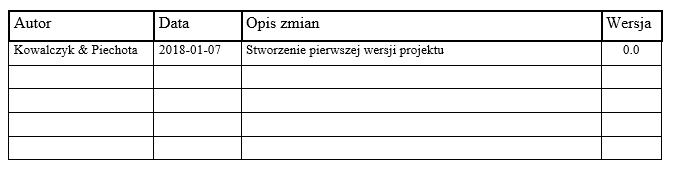
\includegraphics[scale=0.9]{obrazki/postep}
\end{figure}
\end{center}

\newpage

\begin{center}
\begin{figure}[H]
	\centering
	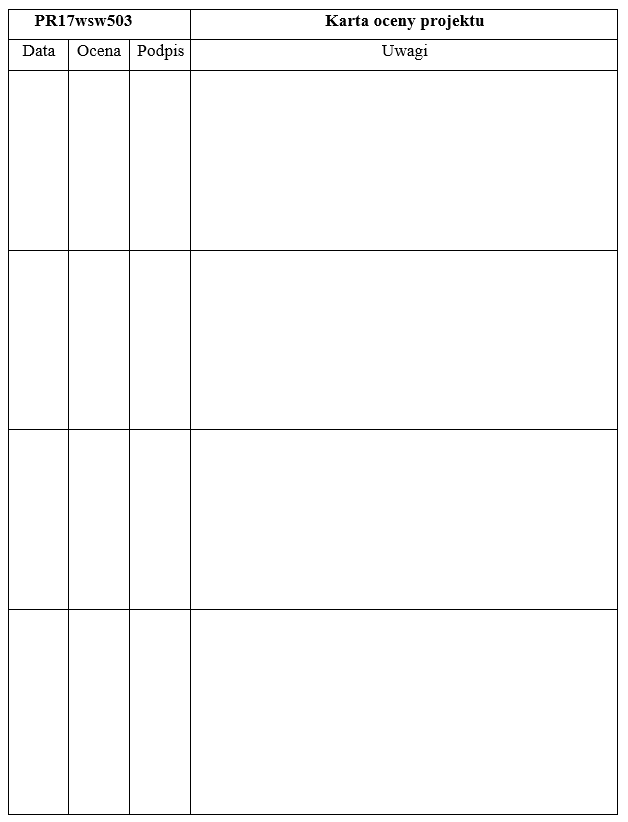
\includegraphics[scale=1]{obrazki/ocena}
\end{figure}
\end{center}

\appendix
\nocite{*}
\printbibliography
\addcontentsline{toc}{section}{Bibliografia}
\end{document}